\section{Zero Field Splitting}\label{zfs}
\index{ZFS}{ZFS} is in fact due to the combined effects of fine structure and a dipole-dipole interaction. These effects manifest themselves identically which makes them difficult to separate experimentally. They each depend on a traceless matrix $D$, as will be shown, which can be totally described by two parameters, conventionally labelled $D$ and $E$. 
For simplicity in this work we will consider the combined effect of both the fine-structure and the dipole-dipole interaction as the ZFS interaction. This means when $D$ and $E$ are measured for a specific system, they represent the compound effect of fine-structure splitting and the dipole interaction, but totally describe the zero-field splitting. 

\begin{figure}[H]
    \begin{center}
        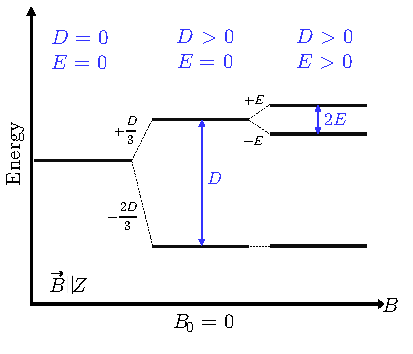
\includegraphics[width=0.6\textwidth]{figures/ZFS.pdf}
    \end{center}
    \caption{Adapted from figure shown in the work by Gr\"{u}ne. }\label{fig:ZFS}
    \todo[inline, color=ediblue]{Write caption}
\end{figure}



\subsection{Fine Structure}
The matrix $D$ in \eqref{eq:fine_structure} has form 
\begin{equation}
   D = \begin{pmatrix}
       D_{xx} & D_{xy} & D_{xz} \\ 
       D_{yx} & D_{yy} & D_{yz} \\ 
       D_{zx} & D_{zy} & D_{zz} \\ 
   \end{pmatrix} 
    % \label{eq:}
\end{equation}
which may be simplified by alignment to the wider system axis and diagonalising the matrix as 
\begin{equation}
   D = \begin{pmatrix}
       D_{xx} & 0 & 0 \\ 
       0 & D_{yy} & 0 \\ 
       0 & 0 & D_{zz} \\ 
   \end{pmatrix}.
    \label{eq:fine_splitting_D}
\end{equation}

The \index{trace}{trace} of the matrix $\text{Tr}(D)$ is unchanged by the change of basis. Since for EPR we are only concerned with the changes in energy and not the absolute, we may choose the value of the trace without any loss of generality, so we set it equal to zero. 
\begin{equation}
    \text{Tr}(D) = 0. 
    % \label{eq:}
\end{equation}

This means that the diagonal form of $D$ may be fully determined by just two parameters 
\begin{eqnarray}
    &D &= D_{zz} - (D_{xx}+ D_{yy})/2 \label{fs_D}\\ 
    &E &= (D_{xx} - D_{yy})/2 \label{fs_E}
\end{eqnarray}

Here $D$ represents the axially symmetric parameter and $E$ represents any non-axial contribution of the fine-structure interaction. 

Substituting \eqref{fs_D} and \eqref{fs_E} into \eqref{eq:fine_structure} and expanding allows us to write our fine-structure Hamiltonian as
\begin{equation}
    H_{\ce{FS}} = D \left(\hat{S}_z^2 - \frac{1}{3}S(S+1)\right) + E\left(\hat{S}_x^2 - \hat{S}_y^2\right).
    \label{eq:fine_structure_hamiltonian}
\end{equation}

\subsection{Dipole-Dipole Interaction}
We will now show that the interaction of the spin of two electrons has the same form as \eqref{eq:fine_structure} by considering two electrons ($S=1/2$). 

Classically, the energy between two magnetic dipoles, $\mu_1, \mu_2$ is calculated as
\begin{equation}
    E = \frac{1}{r^3} \left(\mu_1 \cdot \mu_2 -\frac{3(\mu_1 \cdot \vec{r})(\mu_2 \cdot \vec{r})}{r^2}\right).
    % \label{eq:}
\end{equation}

To uplift the classical expression to quantum mechanics, we substitute the operator representations for the spin induced dipoles 
\begin{equation}
    H_{\ce{DD}} = g_S^2 \mu_B^2 \frac{1}{r^3} \left(\hat{\vec{S}}_1 \cdot \hat{\vec{S}}_2 -\frac{3(\hat{\vec{S}}_1 \cdot \vec{r})(\hat{\vec{S}}_2 \cdot \vec{r})}{r^2}\right).
    % \label{eq:}
\end{equation}

Considering the total spin of the system we may expand this to obtain \cite{carrington1967introduction} 
\begin{equation}
    H_{\ce{DD}} = \frac{1}{2r^5}g_S^2 \mu_B^2 \hat{\vec{S}} \cdot
    \underbrace{
    \begin{pmatrix}
        {r^2 - 3x^2} & -3xy & - 3xz\\ 
        -3xy & r^2 - 3y^2 & -3yz \\ 
        -3xz & -3yz & r^2 - 3z^2 
    \end{pmatrix}
}_{D}
    \cdot \hat{\vec{S}}.
    \label{eq:dd_matrix_form}
\end{equation}

As with \eqref{eq:fine_splitting_D} the matrix $D$ in \eqref{eq:dd_matrix_form} has a constant trace (which we may select to be $0$) leaving the form of the dipole-dipole interaction identical to that of the fine structure interaction 

\begin{equation}
    H_{\ce{DD}} = \hat{\vec{S}} \cdot D \cdot \hat{\vec{S}}.
    % \label{eq:}
\end{equation}

We therefore decompose the traceless matrix $D$ into the axial and non-axial parameters \index{ZFS!$D$}{$D$} and \index{ZFS!$E$}{$E$} as above. 


\subsection{Zero Field Splitting Hamiltonian}
Determining $D$ and $E$ by experiment will yield the combined effect will be contained within those measurements so we may therefore describe the zero field splitting interaction as a whole using 
\begin{equation}
    H_{\ce{ZFS}} =D \left(\hat{S}_z^2 - \frac{1}{3}S(S+1)\right) + E\left(\hat{S}_x^2 - \hat{S}_y^2\right).
    \label{eq:ZFS_hamiltonian}
\end{equation}

The effects of $D$ and $E$ on a triplet state are illustrated in Figure~\ref{fig:ZFS}.


